\documentclass[tikz,border=10pt]{standalone}
\usepackage{tikz}
\usetikzlibrary{calc}

\begin{document}
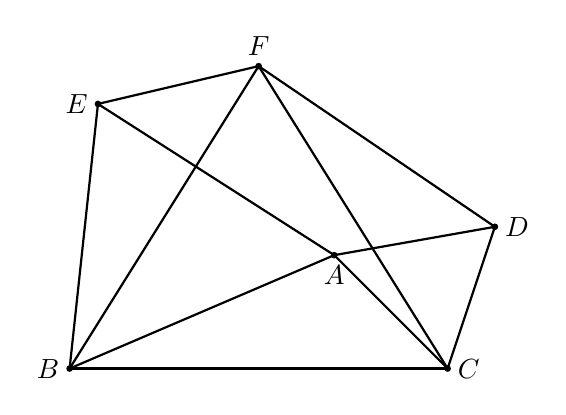
\begin{tikzpicture}[>=stealth, thick, scale=1.2]

    % 1. 定义核心顶点坐标 (基于图像视觉比例)
    \coordinate (B) at (0,0);
    \coordinate (C) at (4,0);
    \coordinate (A) at (2.8,1.2);

    % 2. 计算构造点 (假设存在等边关系或特定比例，此处还原图像形态)
    % E点位于B左上方
    \coordinate (E) at (0.3,2.8);
    % D点位于C右上方
    \coordinate (D) at (4.5,1.5);
    % F点为顶部顶点
    \coordinate (F) at (2,3.2);

    % 3. 绘制实线边框和内部连接线
    % 底部边
    \draw (B) -- (C);

    % 连接 A 的相关线段
    \draw (B) -- (A) -- (C);
    \draw (E) -- (A) -- (D);

    % 连接 F 的相关线段
    \draw (B) -- (F) -- (C);
    \draw (E) -- (F) -- (D);

    % 外部轮廓线
    \draw (B) -- (E);
    \draw (C) -- (D);

    % 4. 绘制顶点并标注字母
    \fill (A) circle (1pt) node[below] {$A$};
    \fill (B) circle (1pt) node[left] {$B$};
    \fill (C) circle (1pt) node[right] {$C$};
    \fill (D) circle (1pt) node[right] {$D$};
    \fill (E) circle (1pt) node[left] {$E$};
    \fill (F) circle (1pt) node[above] {$F$};

\end{tikzpicture}
\end{document}